\documentclass{report}
\usepackage{amsmath}
\usepackage{geometry}
\usepackage{graphicx}
\usepackage{epstopdf}
\begin{document} 

\begin{flushleft}

\begin{Large}

\textbf{Name - Ankush Vijay Israney} \\
\textbf{Student ID - 14057308} \\
\textbf{CS 613 - Assignment 1 report} \\ 

\end{Large}

\break

\underline { \textbf{PART-1}}  \linebreak[2]

\underline {Answer-1}  \linebreak[2]
We like to use quadratic error functions since they allow us to give satisfactory results when it is desired to reach a single minima/maxima in expectation minimization/maximization problems. In a highly dimensional space, for instance if use a 4th degree polynomial function it would provide us with 2 minima/maxima depending on the nature of the curve. But if our goal is to just reach a single minima/maxima instead of a globally optimal one then we would want use a quadratic error function instead of a higher degree polynomial function which would allow us to save computational effort and time and be a good fit to the model of data.
\linebreak[2]


\underline{Answer-2 A} 
\linebreak[2]

Data, X = 

\[\begin{bmatrix}
-2&1 \\
-5&-4 \\
-3&1 \\
0&3 \\
-8&11 \\
-2&5 \\
1&0 \\
5&-1 \\
-1&3 \\
6&1 \\
\end{bmatrix}\] \linebreak[1]

\begin{equation}
\mu_1 = (-2 -5 -3 + 0 -8 -2 + 1 + 5 -1 +6) / 10 = -0.9 
\end{equation}

\begin{equation}
\mu_2 = (1 -4 + 1 + 3 + 11 + 5 + 0 - 1 -3 + 1) / 10 = 1.4
\end{equation}

\begin{equation}
\sigma_1 = \sqrt{\Sigma (x_{i1} - \mu_1) } = 4.011
\end{equation}

\begin{equation}
\sigma_2 = \sqrt{\Sigma (x_{i2} - \mu_2) } = 4.0456
\end{equation}

\begin{equation}
X_{standardized} = \begin{bmatrix}
-0.2601 & -0.0935 \\
-0.9696 & -1.2634 \\
-0.4966 & -0.0935 \\
0.2128 & 0.3743 \\
-1.6791 & 2.2461 \\
-0.26015 & 0.8423 \\
0.4493 & -0.3275 \\
1.3953 & -0.5615 \\
-0.0236 & -1.0294 \\
1.6318 & -0.0935 \\
\end{bmatrix}
\end{equation}

\begin{equation}
\Sigma(X) = \frac{X^TX}{N-1}  
\end{equation}

\[=\begin{bmatrix}
1 & -0.4083 \\
-0.4083 & 1
\end{bmatrix}\]

\begin{equation}
Now, \lambda^2 - \lambda(1+1) + (1-0.167) = \lambda^2 - 2\lambda + 0.833 = 0
\end{equation}

\[
Solving for \lambda, \lambda = 1.4083, 0.5913
\]

\begin{equation}
(\Sigma (X) - \lambda I)x = 0
\end{equation}

\begin{equation}
(\begin{bmatrix}
1 & -0.4083 \\
-0.4083 & 1
\end{bmatrix} - 
\begin{bmatrix}
1.4087 & 0 \\
0 & 1.4087
\end{bmatrix})
\begin{bmatrix}
x \\
y
\end{bmatrix}
= 0, for \lambda = 1.4083
\end{equation} \\

when x =1, y =-1
\[
e1 = \begin{bmatrix}0.7071 & -0.7071\end{bmatrix}^T, normalized
\]

\begin{equation}
(\begin{bmatrix}
1 & -0.4083 \\
-0.4083 & 1
\end{bmatrix} - 
\begin{bmatrix}
0.5913 & 0 \\
0 & 0.5913
\end{bmatrix})
\begin{bmatrix}
x \\
y
\end{bmatrix}
= 0, for \lambda = 0.5913
\end{equation} \\

when x = 1, y = 1
\[
e2 = \begin{bmatrix}0.7071 & 0.7071\end{bmatrix}^T, normalized
\] \linebreak[2]

\underline {Answer-2 B}  \linebreak[2]

Projecting Data Points onto e1, eigen vector with largest magnitude:

Z = XW \linebreak[2]

Therefore,

\[
\begin{bmatrix}
-0.2601 & -0.0935 \\
-0.9696 & -1.2634 \\
-0.4966 & -0.0935 \\
0.2128 & 0.3743 \\
-1.6791 & 2.2461 \\
-0.26015 & 0.8423 \\
0.4493 & -0.3275 \\
1.3953 & -0.5615 \\
-0.0236 & -1.0294 \\
1.6318 & -0.0935 \\
\end{bmatrix}
\times
\begin{bmatrix}0.7071 \\
-0.7071
\end{bmatrix} =
\begin{bmatrix}
2.1213 \\
0.7071 \\
2.8284 \\
2.1213 \\
13.4350 \\
4.9497 \\
-0.7071 \\
-4.2426 \\
-1.4142 \\
-3.5355 \\
\end{bmatrix}
\] \linebreak[2]

\underline {Answer-3 A}  \linebreak[2]

\begin{equation} 
Class 1 = 
\begin{bmatrix}
-2 & 1 \\
-5 & -4 \\
-3 & 1 \\
0 &	3 \\
-8 & 11 \\
\end{bmatrix}
\end{equation}

\begin{equation} 
Class 2 = 
\begin{bmatrix}
-2 & 5 \\
1 & 0 \\
5 & -1 \\
-1 & -3 \\
6 & 1 \\
\end{bmatrix}
\end{equation}

\underline{feature1} 
\[p_0 = 1 ,
p_{-2} = 1 ,
p_{-3} = 1 ,
p_{-5} = 1 ,
p_{-8} = 1 , 
\] 

\[n_{-2} = 1 ,
n_{-1} = 1 ,
n_{1} = 1 ,
n_{5} = 1 ,
n_{6} = 1 , 
\]

Accounting for -2, rest 0
\[
Entropy = \frac{2}{10}*(-\frac{1}{2}*\log_2(\frac{1}{2}) - \frac{1}{2}\log_2(\frac{1}{2})) 
\] 

Entropy = 0.2

\begin{equation}
IG(1) =  -\frac{5}{10}*\log_2(\frac{5}{10})-\frac{5}{10}*\log_2(\frac{5}{10}) -0.2  = 1 - 0.2 = 0.8
\end{equation}

\underline{feature2} 
\[p_1 = 2 ,
p_{-4} = 1 ,
p_{3} = 1 ,
p_{11} = 1 ,
\] 

\[n_{1} = 1 ,
n_{5} = 1 ,
n_{0} = 1 ,
n_{-1} = 1 ,
n_{-3} = 1 , 
\]

Accounting for 1, rest 0
\[
Entropy = \frac{3}{10}*(-\frac{2}{3}*\log_2(\frac{2}{3}) - \frac{1}{3}\log_2(\frac{1}{3})) 
\] 

Entropy = 0.3 * (0.924) = 0.2772

\begin{equation}
IG(1) =  -\frac{5}{10}*\log_2(\frac{5}{10})-\frac{5}{10}*\log_2(\frac{5}{10})  = 1 - 0.2772 = 0.7228
\end{equation}


\underline {Answer-3 B}  \linebreak[2]

Since Information Gain for Feature 1 is more than Information Gain for feature 2, therefore feature 1 seems to be more discriminating.  \linebreak[2]

\underline {Answer-3 C}  \linebreak[2]

\begin{equation} 
Class 1 = 
\begin{bmatrix}
-2 & 1 \\
-5 & -4 \\
-3 & 1 \\
0 &	3 \\
-8 & 11 \\
\end{bmatrix}
\end{equation}

\begin{equation} 
Class 2 = 
\begin{bmatrix}
-2 & 5 \\
1 & 0 \\
5 & -1 \\
-1 & -3 \\
6 & 1 \\
\end{bmatrix}
\end{equation}

\begin{equation}
\mu_1 = \begin{bmatrix}
(-2 -5 -3 + 0 -8)/5 & (1-4+1+3+11)/5 \end{bmatrix} = \begin{bmatrix}-3.6 & 2.4 \end{bmatrix}
\end{equation}

\begin{equation}
\mu_1 = \begin{bmatrix}
(-2 + 1 + 5 - 1 + 6)/5 & (5 + 0 - 1 - 3 + 1)/5 \end{bmatrix} = \begin{bmatrix}1.8 & 0.4 \end{bmatrix}
\end{equation}

\begin{equation}
\Sigma(C1) = \frac{C1^TC1}{N-1}  
\end{equation}

\[=\begin{bmatrix}
9.30 & -7.45 \\
-7.45 & 29.80
\end{bmatrix}\]

\begin{equation}
\Sigma(C2) = \frac{C2^TC2}{N-1}  
\end{equation}

\[=\begin{bmatrix}
12.70 &	-2.40 \\
-2.40 &	8.80
\end{bmatrix}\]


\begin{equation}
\sigma_1^2 = (5-1)*\Sigma(C1) = 4 * \begin{bmatrix}
9.30 & -7.45 \\
-7.45 & 29.80
\end{bmatrix} = \begin{bmatrix}
37.20 &	-29.80 \\
-29.80 & 119.20
\end{bmatrix}
\end{equation}

\begin{equation}
\sigma_2^2 = (5-1)* \Sigma(C2) = 4 * \begin{bmatrix}
12.70 &	-2.40 \\
-2.40 &	8.80
\end{bmatrix} = \begin{bmatrix}
50.80 &	-9.60 \\
-9.60 &	35.20
\end{bmatrix}
\end{equation}

\begin{equation}
S_b = (\mu_1 - \mu2)^T*(\mu1_ - \mu_2) = (\begin{bmatrix}3.6 & 2.4 \end{bmatrix}
- \begin{bmatrix}1.8 & 0.4 \end{bmatrix})^T
\times
(\begin{bmatrix}-3.6 & 2.4 \end{bmatrix}
- \begin{bmatrix}1.8 & 0.4 \end{bmatrix})
=
\begin{bmatrix}-5.4 \\
2.0
 \end{bmatrix}
 \times
\begin{bmatrix}-5.4 & 2.0
 \end{bmatrix}  
\end{equation}

\[
=\begin{bmatrix}
 29.16 & -10.80 \\
-10.80 &	4.0
\end{bmatrix}
\]

\begin{equation}
S_w = \Sigma^2 + \Sigma^2 = \begin{bmatrix}
37.20 &	-29.80 \\
-29.80 & 119.20
\end{bmatrix} +
 \begin{bmatrix}
50.80 &	-9.60 \\
-9.60 &	35.20
\end{bmatrix} = 
\begin{bmatrix}
88	& -39.40 \\
-39.40 & 154.40
\end{bmatrix}
\end{equation}

\begin{equation}
S_w = \Sigma^2 + \Sigma^2 = \begin{bmatrix}
37.20 &	-29.80 \\
-29.80 & 119.20
\end{bmatrix} +
 \begin{bmatrix}
50.80 &	-9.60 \\
-9.60 &	35.20
\end{bmatrix} = 
\begin{bmatrix}
88	& -39.40 \\
-39.40 & 154.40
\end{bmatrix}
\end{equation}

\begin{equation}
S_w^{-1} = \frac{1}{12035} * \begin{bmatrix}
154.40 & 39.40 \\
39.40 & 88
\end{bmatrix}
=\begin{bmatrix}
0.0128 & 0.0033 \\
0.0033 & 0.0073
\end{bmatrix}
\end{equation}

\begin{equation}
X = S_w^{-1}*S_b = \begin{bmatrix}
0.0128 & 0.0033 \\
0.0033 & 0.0073
\end{bmatrix}
\times
\begin{bmatrix}
 29.16 & -10.80 \\
-10.80 &	4.0
\end{bmatrix}
= 
\begin{bmatrix}
0.3387 & -0.1254 \\
0.0165 & -0.0061
\end{bmatrix}
\end{equation}


\begin{equation}
Now, \lambda^2 - \lambda(0.3326) + (-0.002-0.002) = \lambda^2 - 0.3326\lambda = 0
\end{equation}

\[
Solving for \lambda, \lambda = 0.3326, 0
\]

\begin{equation}
(\Sigma (X) - \lambda I)x = 0
\end{equation}

\begin{equation}
(\begin{bmatrix}
0.3387 & -0.1254 \\
0.0165 & -0.0061
\end{bmatrix} - 
\begin{bmatrix}
0.3326 & 0 \\
0 & 0.3326
\end{bmatrix})
\begin{bmatrix}
x \\
y
\end{bmatrix}
= 0, for \lambda = 0.3326
\end{equation} \\

when x =1, y =0.04 \\
\[
e2 = \begin{bmatrix}0.9988 & 0.0486\end{bmatrix}^T, normalized
\] \linebreak[2]

\begin{equation}
(\begin{bmatrix}
0.3387 & -0.1254 \\
0.0165 & -0.0061
\end{bmatrix} - 
\begin{bmatrix}
0 & 0 \\
0 & 0
\end{bmatrix})
\begin{bmatrix}
x \\
y
\end{bmatrix}
= 0, for \lambda = 0
\end{equation} \\

e2 not to be considered (zero magnitude) \linebreak[2]

\underline {Answer-3 D}  \linebreak[2]

Projecting Data Points onto e1, eigen vector with largest magnitude (unit length):

Z1 = C1*W \linebreak[2]

Therefore,

\[
\begin{bmatrix}
-2 & 1 \\
-5 & -4 \\
-3 & 1 \\
0 &	3 \\
-8 & 11 \\
\end{bmatrix}
\times
\begin{bmatrix} 0.9988 \\
 0.0486
\end{bmatrix} =
\begin{bmatrix}
-0.66527 \\
-1.66319 \\
-0.9979 \\
0 \\
-2.6611 \\
\end{bmatrix}
\] \linebreak[2]

Z2 = C2*W \linebreak[2]

Therefore,

\[
\begin{bmatrix}
-2 & 5 \\
1 & 0  \\
5 & -1 \\
-1 & -3 \\
6 & 1 \\
\end{bmatrix}
\times
\begin{bmatrix} 0.9988 \\
 0.0486
\end{bmatrix} =
\begin{bmatrix}
-0.66527 \\
0.3326 \\
1.6631 \\
-0.3326 \\
1.9958 \\
\end{bmatrix}
\] \linebreak[2]

\underline {Answer-3 E}  \linebreak[2]
If we consider that we are projecting the points from 2 dimensions to 1 dimension then we can say that the projection from the previous part seems to provide some decent class separation. In Class 1, 3 out of the 5 points are on the negative scale of the axis and in Class 2, 3 out of the 5 points are on the positive scale of the axis.
However, one of the points (-0.66527) is directly coinciding and 1 point (-0.3326) in Class 2 crosses and seems to be as a part of class 1. Therefore, I would say that the nature of the data cannot be clearly separable in a 1D space and we probably could do better when we consider a higher dimensional space. \linebreak[2]

\break
\underline { \textbf{PART-2}}  \linebreak[2]

\begin{figure}[tph!]
\centering
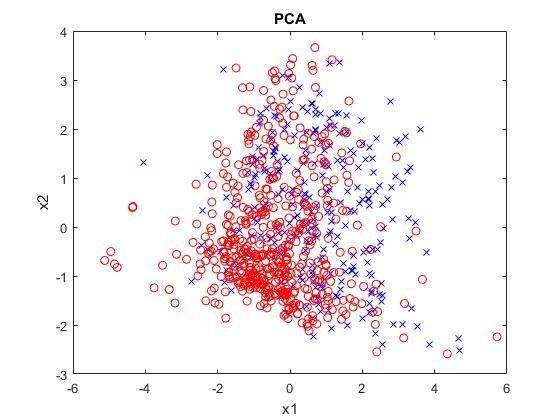
\includegraphics{part2.jpg}
\end{figure}

\break
\underline { \textbf{PART-3 - It took 27 iterations for the algorithm to terminate}}\linebreak[2]

\begin{figure}[tph!]
\centering
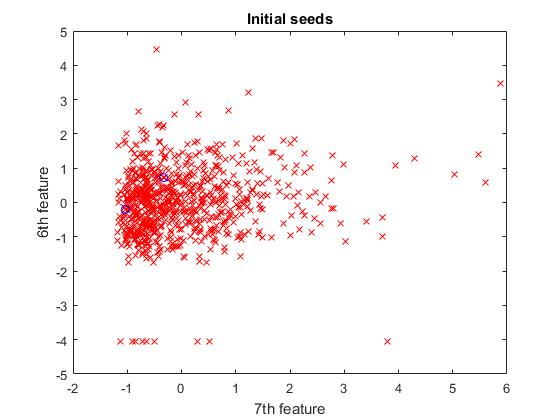
\includegraphics{part3seeds.jpg}
\end{figure}

\begin{figure}[tph!]
\centering
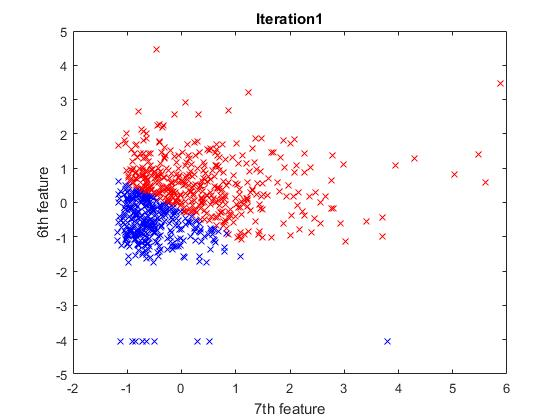
\includegraphics{iteration1.jpg}
\end{figure}

\begin{figure}[tph!]
\centering
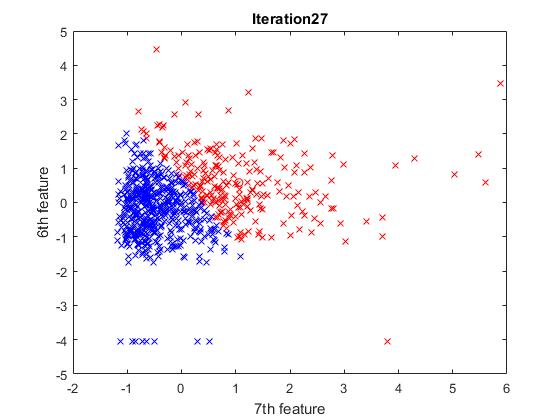
\includegraphics{iterationn.jpg}
\end{figure}

\end{flushleft} 

\end{document}